\subsection{Shadows}\label{sec:shadowsexperiment}

In the Unity3D[ref] engine there are a number of way to light an environment, each way also has its own limitations when calculating shadows in the environment. Following will be experimentation and analysis of these lighting method will be carried out, to figure out which method is most useful for our use case. 


Directional lighting method uses a orthographic projection from the light source position and direction of the scene, whereas the two other methods uses at perspective projection with a full 360 degree field of view for point but a variable projection angle for spotlight within the range (0,180), The shadows are compiled as shadow maps as described by \cite{Wimmer2004}, the differing amount pixelation between the types of lighting method, we will see, is explained by the individual methods varying maximum shadow map sizes\cite{unityshadowmapsize}.

\begin{figure}
\centering
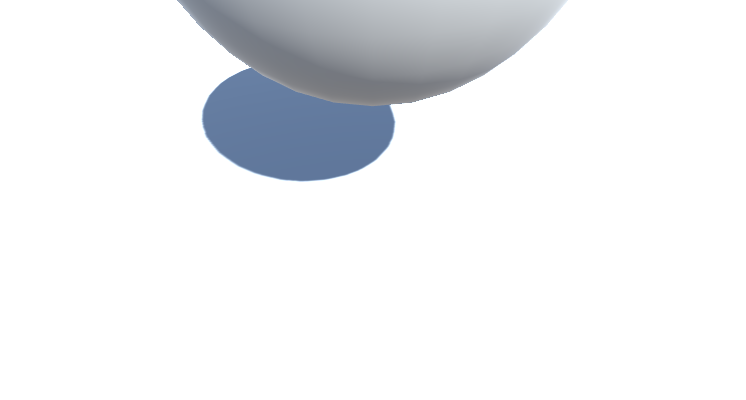
\includegraphics[width=\linewidth]{figures/shadows/directional-cleaned}
\caption{directional}
\label{fig:directional}
\caption{
The directional lighting of \cite{unitylighttypes}.
}
\end{figure}

First off for the most realistic lighting where the lighting is coming from a single center point, like a light bulb, the perspective projections are preferred\cite{unitylighttypes}, which means that the orthographic projections of the directional light, fig.~\ref{fig:directional}, is not a good approximation. However the directional lighting gave the best overall result in terms of the resolution of the shadows.

\begin{figure}
\begin{subfigure}[t]{0.5\textwidth}
\centering
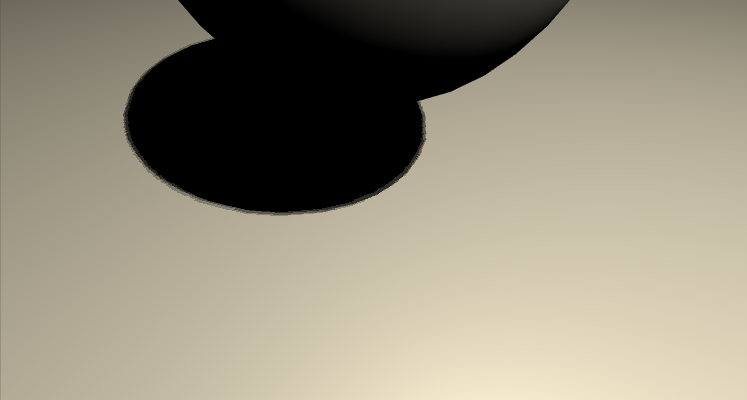
\includegraphics[width=\linewidth]{figures/shadows/point-cleaned}
\caption{point}
\label{fig:point}
\end{subfigure}%
    \hfill
\begin{subfigure}[t]{0.5\textwidth}
\centering

\includegraphics[width=\linewidth]{figures/shadows/point-far-cleaned}
\caption{point far}
\label{fig:point-far}
\end{subfigure}
\caption{The two variations of point light, (a) point up close to the object casting the shadow and (b) far from the object.}
\end{figure}

Up close to the target and its backdrop surface we see that the point light, fig.~\ref{fig:point} gives us tight fit silhouette shadow but it has a pixelated gradient near the edges. From a far distance, fig.~\ref{fig:point-far} the shadow just disappears but of the low maximum resolution of the shadow map.

\begin{table}
  \centering
  \begin{tabular}{| c | c | c | }
    \hline
    & Close & Far \\ \hline
    Narrow &  \begin{minipage}{.5\textwidth}
            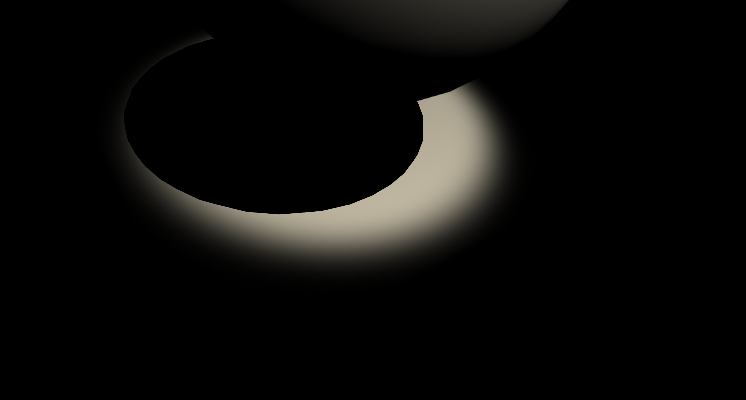
\includegraphics[width=\linewidth]{figures/shadows/spot-cleaned}
            \end{minipage}
            &
            \begin{minipage}{.5\textwidth}
            
\includegraphics[width=\linewidth]{figures/shadows/spot-far-cleaned}
            \end{minipage}
    \\ \hline
    Wide &  \begin{minipage}{.5\textwidth}
            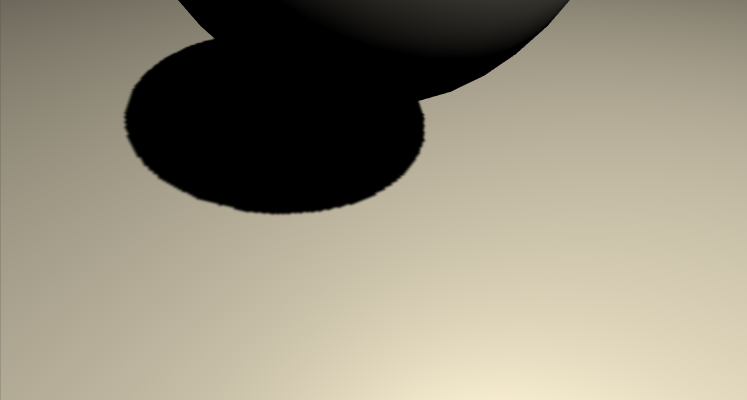
\includegraphics[width=\linewidth]{figures/shadows/spot-wide-cleaned}
            \end{minipage}
            &
            \begin{minipage}{.5\textwidth}
            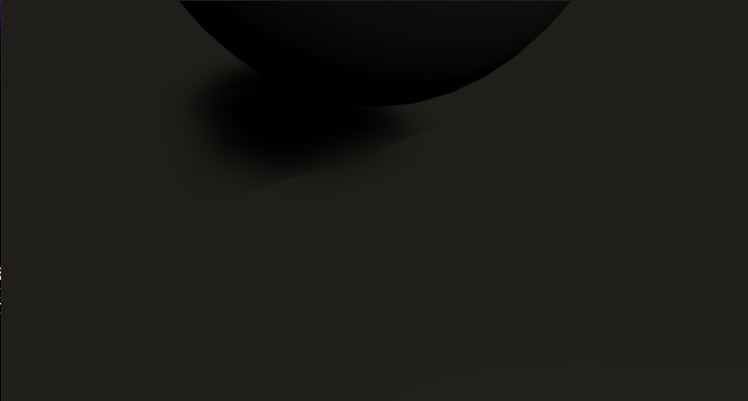
\includegraphics[width=\linewidth]{figures/shadows/spot-wide-far-cleaned}
            \end{minipage}
    \\ \hline
    Widest &  
            \begin{minipage}{.5\textwidth}
            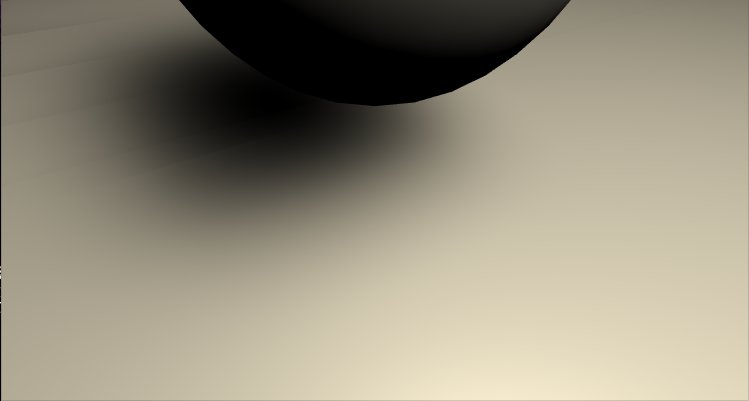
\includegraphics[width=\linewidth]{figures/shadows/spot-widest-cleaned}
            \end{minipage}
            &
            \begin{minipage}{.5\textwidth}
            
\includegraphics[width=\linewidth]{figures/shadows/spot-widest-far-cleaned}
            \end{minipage}
    \\ \hline
  \end{tabular}
  \caption{Spot lights in differing setups}\label{tbl:spot-analysis}
\end{table}

In figure ~\ref{tbl:spot-analysis} we can observer that even with a wide angle the spot light produces reasonable results with sharp edges up close and blurry from a far but still occuring. It was concluded that specifically tuned spotlight for each scene was the approach to use for the most realistic shadows.